% Documento técnico (entrega final). Estrutura prescrita pelo enunciado, secção 5.5.
% Compilar: latexmk -pdf relatorio.tex
\documentclass[a4paper,11pt]{article}
\usepackage[T1]{fontenc}
\usepackage[portuguese]{babel}
\usepackage[a4paper,margin=2.5cm]{geometry}
\usepackage{graphicx}
\usepackage[hidelinks]{hyperref}
% \usepackage{pdfpages}   % descomentar para juntar os anexos em PDF

% Diagramas: renderizar os .puml (ex.: plantuml -tpdf) e incluir com \includegraphics.
% \graphicspath{{../../modelos/}}

\begin{document}

% ---------------------------------------------------------------- Capa
\begin{titlepage}
  \centering
  {\large Universidade do Minho --- Licenciatura em Engenharia Informática\par}
  \vspace{1cm}
  {\Large Desenvolvimento de Sistemas de Software\par}
  {\large 2026/2027\par}
  \vspace{2cm}
  {\LARGE\bfseries Grupo NN\par}
  \vspace{1.5cm}
  % Um elemento por caixa: substituir pela fotografia (\includegraphics[height=3.5cm]{...}).
  \fbox{\parbox[c][3.5cm][c]{2.8cm}{\centering foto\\Nome\\Nº}}\hspace{0.3cm}
  \fbox{\parbox[c][3.5cm][c]{2.8cm}{\centering foto\\Nome\\Nº}}\hspace{0.3cm}
  \fbox{\parbox[c][3.5cm][c]{2.8cm}{\centering foto\\Nome\\Nº}}
  \vfill
  Repositório: \url{https://github.com/LEI-DSS/...}
\end{titlepage}

\tableofcontents
\newpage

% ------------------------------------------------- Resultados obtidos
\section{Descrição dos resultados obtidos}
% Máximo uma página.

% ------------------------------------------------ Análise de requisitos
\section{Análise de requisitos}
\subsection{Modelo de domínio}
\subsection{Diagramas de use case}
\subsection{Descrição dos use cases}

% ------------------------------------------------ Modelação conceptual
\section{Modelação conceptual da solução}
\subsection{Diagramas de classes}
\subsection{Diagramas de sequência}

% ------------------------------------------------ Solução implementada
\section{Solução implementada}
\subsection{Diagramas de classes}
\subsection{Diagramas de sequência}
\subsection{Diagrama de componentes}
\subsection{Diagrama de packages}

% ------------------------------------------------ Decisões
\section{Registo de decisões e exclusões}
% Versão final de docs/decisoes.md.

% ------------------------------------------------ Alteração de requisitos
\section{Incorporação da alteração de requisitos}
% Máximo uma página: o que teve de ser alterado.

% ------------------------------------------------ Manual
\section{Manual de utilização}

% ------------------------------------------------ Anexos
\appendix
\section{Enunciado}
% 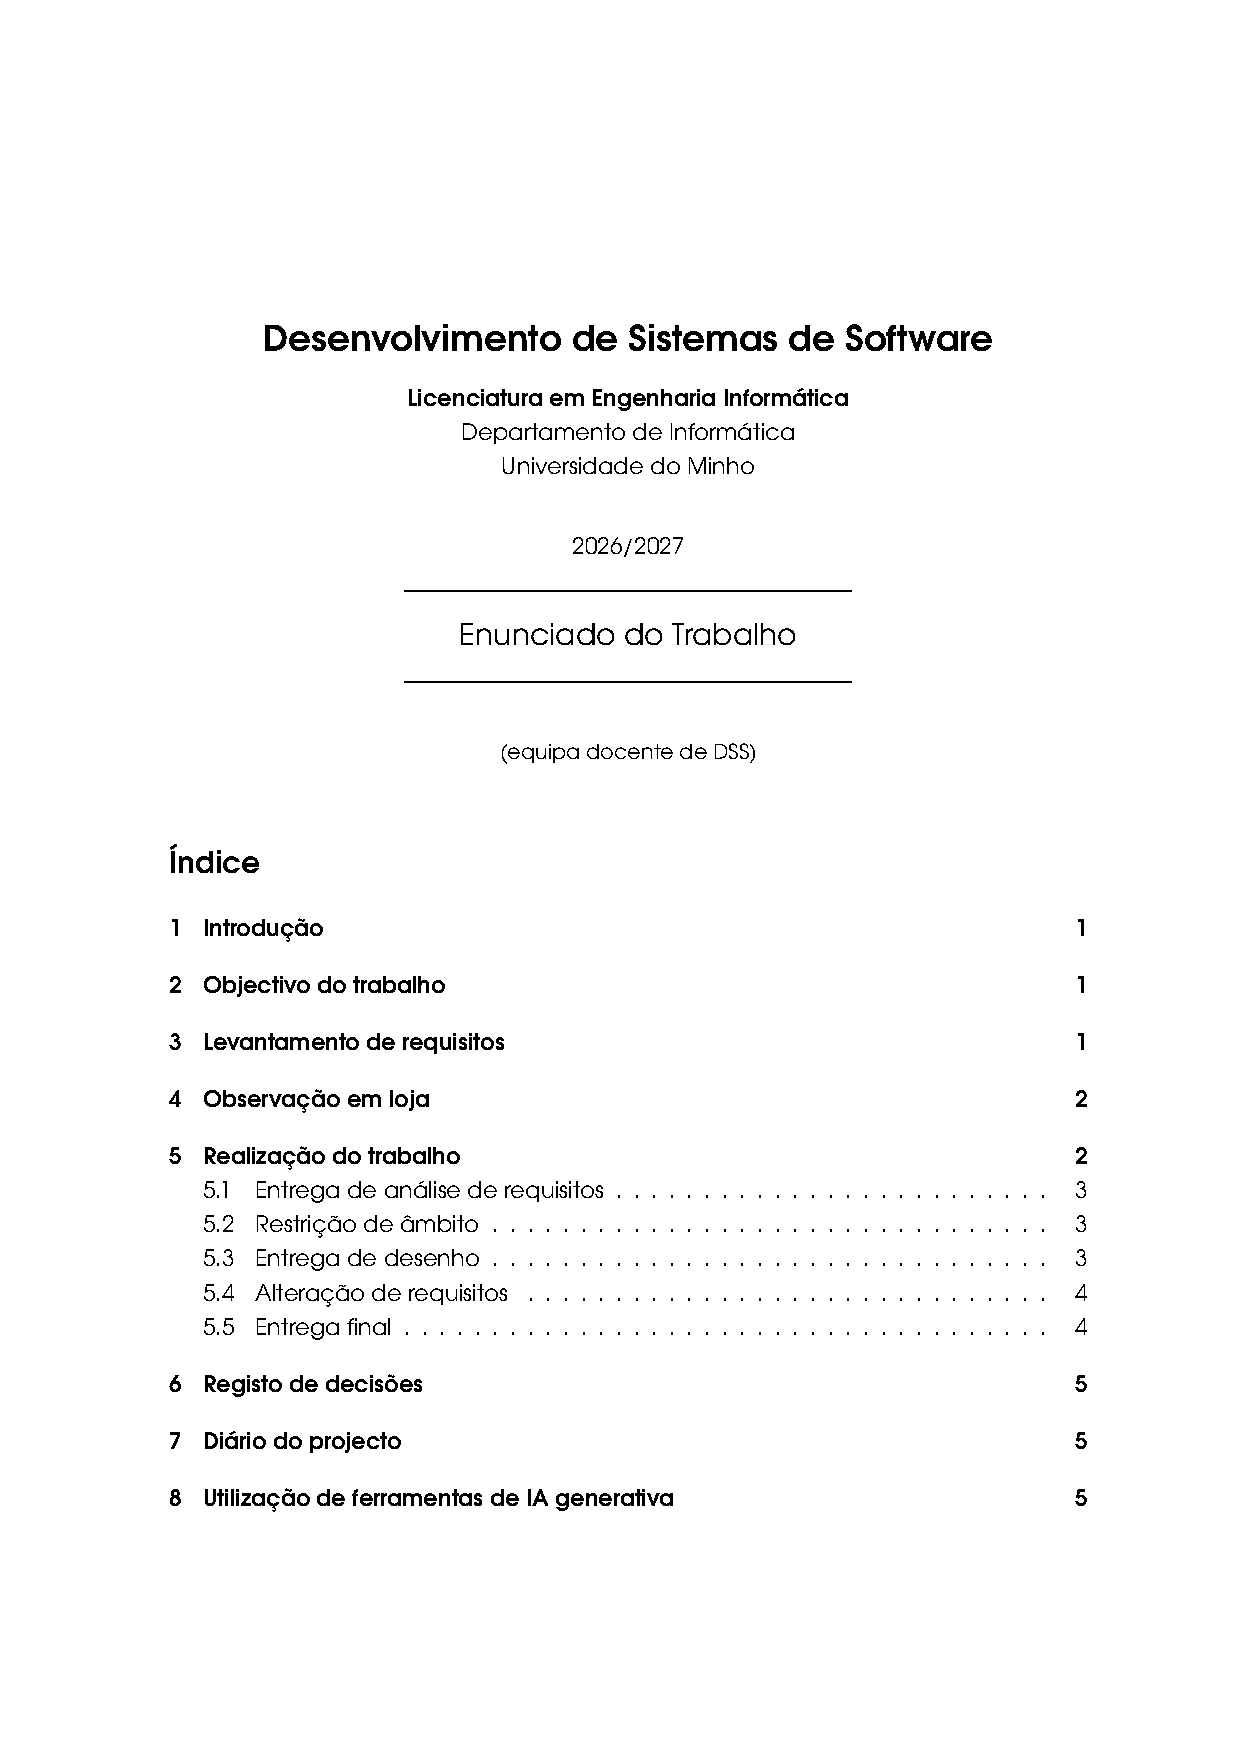
\includepdf[pages=-]{../enunciado/Trabalho_DSS_2026.pdf}
\section{Documento de restrição de âmbito}
% \includepdf[pages=-]{../enunciado/<restricao-de-ambito>.pdf}

\end{document}
